Here we expect to cover a mix of some technical metrics of the system and the \textit{case study} on Dybbølsbro. 
For the former, we expect to cover the precision of OpenDataCam (including YOLO4) with stats such as

\begin{itemize}
	\item Share of bicycles detected (\%)
	\item Mean and median trajectory length
	\item For all frames a bike is visible (and detected at least once), what share of them was the bike detected.
\end{itemize}

which are all compared to the "ground truth" dataset that we annotate manually. We know from previous works with OpenDataCam
that vehicle detection has achieved 95\% accuracy while performing worse for pedestrians and motorcycles (\cite{BROEKMAN2021100068}).

\ \\
On the Dybbølsbro study, we will focus on how well it reproduces the real-world trajectories (desire lines) that
we observe. While the desire line analysis report of Dybbølsbro (from Copenhagenize) is gone, it is from 2014, and many changes have happened since.
We may apply the system to an intersection at Holmens Kanal, as a report is available. Although from 2015, it is a good benchmark to compare against. 


\raggedbottom
\ \\ 
\noindent
\begin{tabular}{@{}cc}
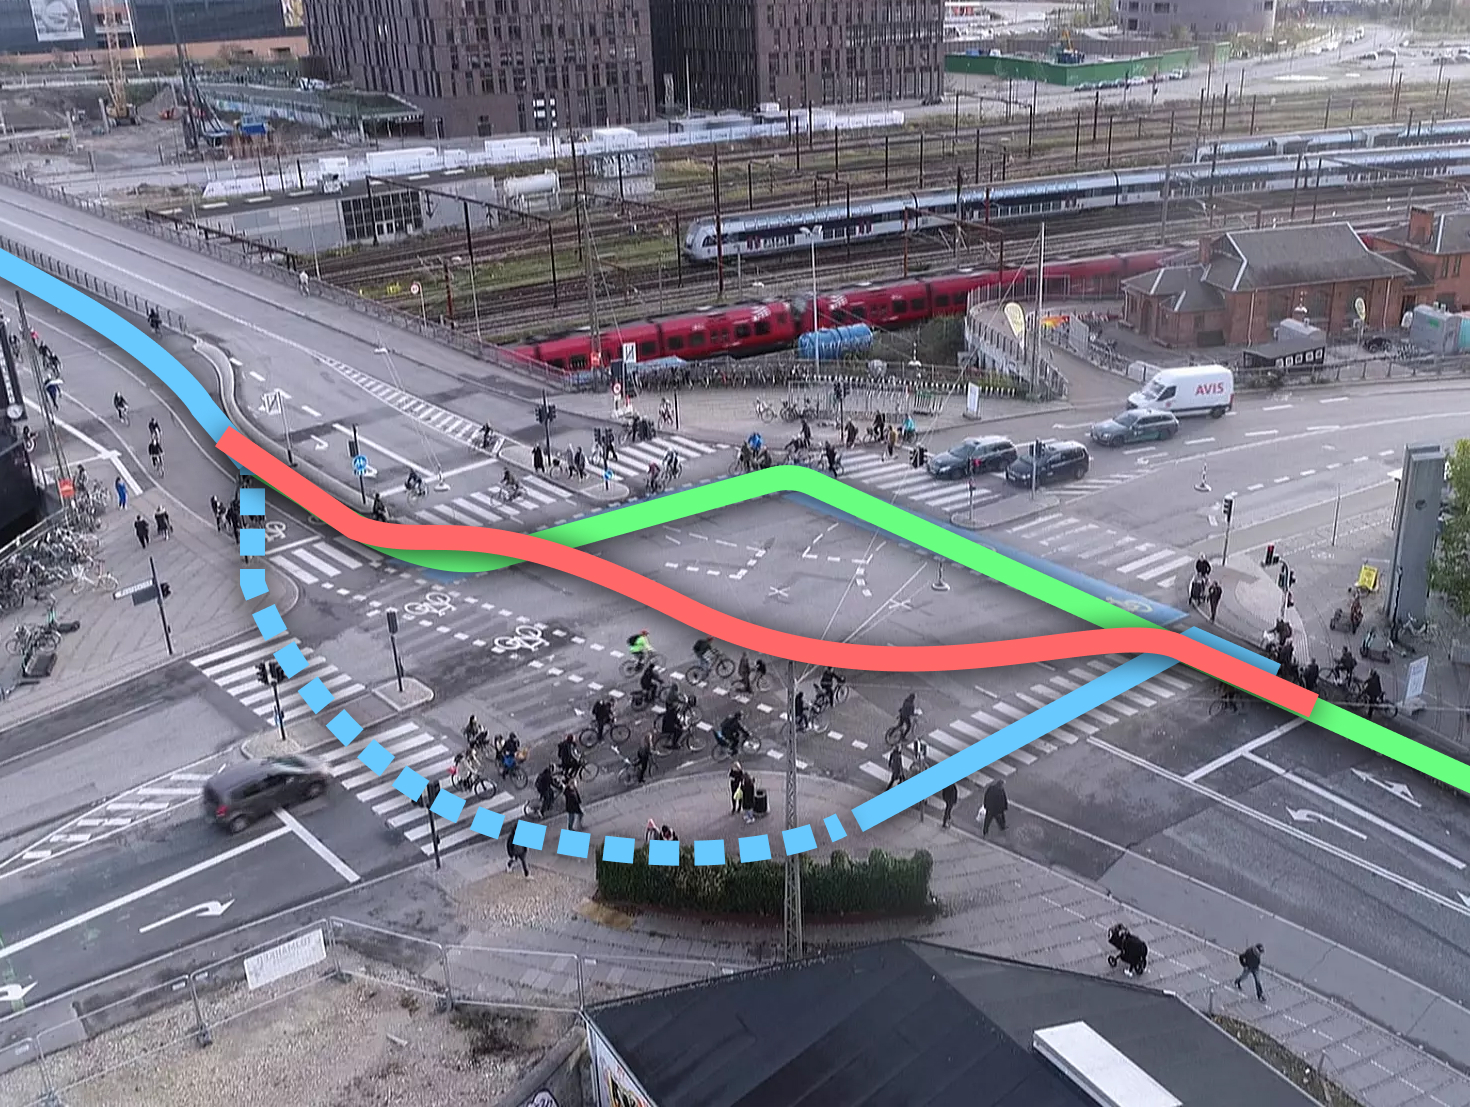
\includegraphics[width=1.0\columnwidth]{paths} 
\end{tabular}
\captionof{figure}{Common trajectories of cyclists comming from NW}